\documentclass{article}
\usepackage{amsmath,amsthm,amssymb,amsfonts}
\usepackage{setspace,enumitem}
\usepackage{graphicx}
\usepackage{hyperref}
\usepackage{natbib}
\usepackage{afterpage}
\usepackage{xcolor}
\usepackage{etoolbox}
\usepackage{booktabs}
\usepackage{pdfpages}
\usepackage{multicol}
\usepackage{geometry}
\usepackage{accents}
\usepackage{bbm}
\usepackage{placeins}
\hypersetup{
	colorlinks,
	linkcolor={blue!90!black},
	citecolor={red!90!black},
	urlcolor={blue!90!black}
}

\newtheorem{theorem}{Theorem}
\newtheorem{assumption}{Assumption}
\newtheorem{definition}{Definition}
\newtheorem{lemma}{Lemma}
\setlength{\parindent}{0cm}
\geometry{margin = 1in}

\newcommand{\R}{\mathbb{R}}
\newcommand{\ubar}[1]{\underaccent{\bar}{#1}}
\newcommand{\Int}{\text{Int}}
\newcommand{\xbf}{\mathbf{x}}
\newcommand{\Abf}{\mathbf{A}}
\newcommand{\Bbf}{\mathbf{B}}
\newcommand{\Gbf}{\mathbf{G}}
\newcommand{\bbf}{\mathbf{b}}
\newcommand{\one}{\mathbbm{1}}

\newtoggle{extended}
\settoggle{extended}{false}

\title{ECON 810: Homework 2}
\author{Alex von Hafften }

\begin{document}

\maketitle

\begin{itemize}

\section{Data}

\item I use the PSID with the following filters:

\begin{itemize}
\item Main sample, no SEO oversample.
\item Observations between 1978 and 1997, inclusive.
\item Ages 25 to 26, inclusive.
\end{itemize}

\item To define the job loss indicator:

\begin{itemize}
\item Dropping observations with lagged hours by one, two, and three periods under 1800 hours (=(52 weeks $-$ 2 weeks vacation) $\times$ 36 hours per week.
\item Dropping observations with lag size not equal to current size.
\item Job loss indicator is one if as hours in the current period being less than 75 percent of the average number of hours in the last three periods.
\end{itemize}

\item The resulting sample has 26,107 observations without job loss and 2,278 observations with job loss.

\item I then estimate a distributed lag regression around job loss.  The coefficients on job losses are plotted in the figure below.

\begin{itemize}
\item There's evidence of a pre-trend with the coefficients statistically significantly negative, around between negative \$2,000 to \$4,000.  I think this pre-trend is likely due to not limiting our analysis to ``mass layoffs" like Davis and von Wachter that can be identified using an employee-employer matched dataset.  We're capturing all job losses, so it reasonable to suspect that losing a job might not be a fully exogenous event.
\item The drop in earning from the period before job loss $k = -1$ to the period after job loss $k = 1$ is about \$9,700.  This estimate is smaller than Davis and von Wachter's estimate for both an expansion and a recession. I think this estimate being smaller could also be due to the definition of job loss being ``less exogenous" here than in Davis and von Wachter.  Indeed, the estimate after job loss $k=1$ relative to the control group is about \$14,100, which is more in align is Davis and von Wachter's estimates.

\end{itemize}

\item See \texttt{part\_1.R} for implementation.

\end{itemize}

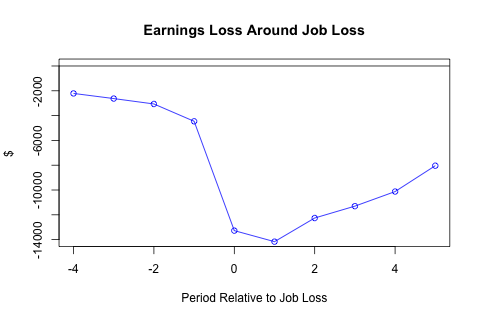
\includegraphics{part_1.png}

\pagebreak

\section{Model}

Since the matching function $M$ is CRS, we can rewrite the job finding rate and the hiring rate in terms of market tightness $\theta \equiv \frac{v}{u}$ where $v$ is vacancies and $u$ is applicants. The job-finding rate becomes:

\begin{align*}
p(\theta) = \frac{M(u, v)}{u} = M(1, \frac{v}{u}) = M(1, \theta) = \frac{\theta}{(1+\theta^\zeta)^{1/\zeta}}
\end{align*}

The hiring rate becomes:

\begin{align*}
p_f(\theta) = \frac{M(u, v)}{v} =M( \frac{u}{v}, 1) = M(\theta^{-1}, 1) = \frac{\theta^{-1}}{(\theta^{-\zeta}+ 1)^{1/\zeta}} = \frac{1}{(1+\theta^\zeta)^{1/\zeta}}
\end{align*}

The inverse of the hiring rate is:

\begin{align*}
\theta(p_f) = (p_f^{-\zeta} - 1)^{1/\zeta}
\end{align*}

\begin{enumerate}

\item Write down the definition of equilibrium for this economy.

...
 
\item Prove that the equilibrium is \textit{Block Recursive}.

...

\item Solve the model above using the suggested parameters and report the following:

\begin{enumerate}

\item Make a histogram of the distribution of assets from your simulated data.

...

\item Make a histogram of the distribution of wages from your simulated data.

...

\item What is the unemployment rate in your economy?

...

\item Plot average earnings and assets over the life-cycle from your model. How do the earnings data compare to your age earnings profile from the PSID?

...

\item In your simulated data, what is the average gain in earnings when employed? How does this compare to your data estimate from last week?s assignment?

...

\item In your simulated data, make a graph of earnings around job loss (following an individual for 4 quarters before job loss to 8 quarters after job loss). How does the graph compare to the estimates from Davis and von Wachter and your estimates from part of the assignment?

...

\item In your simulated data, make a graph of consumption around job loss.

...

\item Increase the transfer to the unemployed by 10\%. How do the above graphs of earnings and consumption around job loss change? What happens to the unemployment rate in your economy?

...

\end{enumerate}

\end{enumerate}

\end{document}

